\documentclass{article}
\usepackage{tikz, comment}
\usepackage{pifont}
\usepackage{fontspec}
\usetikzlibrary{arrows, decorations.markings, decorations.pathreplacing}
\begin{comment}
:Title: Not defined yet
:Slug: No name yet

Description Here.........
\end{comment}
\begin{document}\centering 

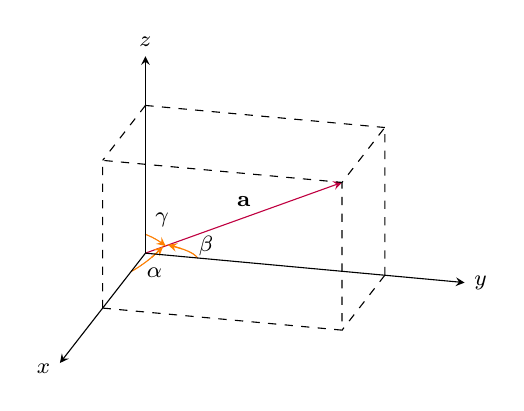
\begin{tikzpicture}[font=\footnotesize]

\pgfplotsset{
    colormap/outside/.style={
        colormap=
            {outside}{
            rgb255(0cm)=(110,110,255);
            rgb255(1cm)=(20,20,255);
            }
    },
    colormap/outside,
    colormap/inside/.style={
        colormap={inside}{
            rgb255(0cm)=(20,20,255);
            rgb255(1cm)=(220,220,255);
        }
    },
    colormap/inside
}

\pgfplotsset{compat=1.8}
\begin{axis}
[axis lines = center, view={105}{30}, ticks = none, scale=0.75,
axis on top, xlabel = {$x$}, ylabel ={$y$}, zlabel ={$z$}, domain =0:1, y domain =0:1,
xmin =0,
xmax =6,
ymin =0,
ymax =8,
zmin =0, 
zmax =12,
samples =10, samples y =40, z buffer =sort, 
every axis x label/.style={
    at={(ticklabel* cs:1)},
    anchor= east, yshift =-2
},
every axis y label/.style={
    at={(ticklabel* cs:1)},
    anchor= west,
},
every axis z label/.style={
    at={(ticklabel* cs:1)},
    anchor= south
},]

\addplot3[purple, ->, >=stealth] coordinates
        {(0,0,0) (3,6,9)};

\addplot3[dashed] coordinates
        {(3,0,0) (3,6,0) (3,6,9)};
\addplot3[dashed] coordinates
        {(3,6,9) (3,0,9) (3,0,0)};  
\addplot3[dashed] coordinates
        {(0,0,9) (0,6,9)};
\addplot3[dashed] coordinates        
        {(0,0,9) (3,0,9)};        
\addplot3[dashed] coordinates        
        {(3,6,9) (0,6,9) (0,6,0)};
\addplot3[dashed] coordinates    
        {(0,6,0) (3,6,0)}; 

    \addplot3 [
      surf,
      domain=0:0.534522,
      samples=15,
      y domain=0:1,
      samples y=2,
      line join=round, 
      mesh/interior colormap name=inside,
      colormap/outside,
      shader=faceted,
      variable=\t,
      point meta={cos(t)},
      faceted color=orange, opacity=1
    ]
           ({sqrt(1^2-t^2-(9/6*t)^2)}, {t}, {9/6*t});
\addplot3[<-, >=stealth, orange] coordinates
{ (0.69282, 0.4, 0.6) (0.267264, 0.534522, 0.801783) };
\node[label={-90:{$\alpha$}}] at (axis cs:0.2, 0.3, 0.6) {};

    \addplot3 [
      surf,
      domain=0:0.347443,
      samples=15,
      y domain=0:1,
      samples y=2,
      line join=round, 
      mesh/interior colormap name=inside,
      colormap/outside,
      shader=faceted,
      variable=\t,
      point meta={cos(t)},
      faceted color=orange, opacity=1
    ]
           ({t}, {sqrt(1.3^2-t^2-(9/3*t)^2)}, {9/3*t});
\addplot3[->, >=stealth, orange] coordinates
{ (0.26, 1.00698, 0.78) (0.347443, 0.694879, 1.04232) };
\node[label={0:{$\beta$}}] at (axis cs:0.15, 0.9, 0.8) {};

    \addplot3 [
      surf,
      domain=1.15:0.92205,
      samples=15,
      y domain=0:1,
      samples y=2,
      line join=round, 
      mesh/interior colormap name=inside,
      colormap/outside,
      shader=faceted,
      variable=\t,
      point meta={cos(t)},
      faceted color=orange, opacity=1
    ]
           ({sqrt((1.15^2-t^2)/5)}, {6/3*sqrt((1.15^2-t^2)/5)}, {t});
\addplot3[->, >=stealth, orange] coordinates
{ (0.289828, 0.579655, 0.95) (0.307354, 0.6147, 0.92205) };
\node[label={90:{$\gamma$}}] at (axis cs:0.253969, 0.507937, 0.8) {};

\node[label={90:{${\bf a}$}}] at (axis cs:1.5, 3, 4) {};
                             
\end{axis}

\end{tikzpicture}
\end{document}